\documentclass{article}
\usepackage[utf8]{inputenc}

\title{BREWDAY!\\
DOCUMENTAZIONE}
\author {- Mazzucchetti Patrick\\ 
- Galbusera Riccardo\\
- Cortez Angelica\\
- Brunelli  Lorenzo
}
\date{Progetto Anno: 2020/2021}
\usepackage{natbib}
\usepackage{graphicx}
\usepackage{geometry}
\geometry{a4paper, top=3cm, bottom=3cm, left=3.5cm, right=3.5cm}
\renewcommand*\contentsname{Summary}
\begin{document}
\maketitle
\clearpage
\tableofcontents
\break
\section{Introduzione}
Progetto del gruppo: Gruppo-Birra-2\\
Brew Day! è un’applicazione fornita in cloud secondo il modello SAAS (Software as a service) che permette ad ogni “beer enthusiasts“ di gestire
la propria produzione di birra artigianale.\\
L’applicazione permette in modo semplice ed intuitivo ad ogni utente registrato di salvare, organizzare e tenere traccia delle proprie ricette, degli
ingredienti utilizzati e della loro disponibilità nella propria dispensa e degli strumenti che ha a disposizione per produrre la propria birra.\\
\clearpage
\subsection{Link Utili}
\subsubsection{Repository Github}
https://github.com/UnimibSoftEngCourse2021/progetto-birra-2-gruppo-birra-2/
\subsubsection{Repository Dockerhub}
\begin{itemize}
\item Backend: https://hub.docker.com/repository/docker/gruppobirra2/brewday
\item Frontend: https://hub.docker.com/repository/docker/gruppobirra2/brewday-frontend
\item MaximizeBrew: https://hub.docker.com/repository/docker/gruppobirra2/maximizebrewtoday
\end{itemize}
\subsection{Jira e Confluence}
 https://progetto-is.atlassian.net/
\subsection{Console AWS}
https://progetto-is.signin.aws.amazon.com/console
\subsection{Sonarcloud}
https://sonarcloud.io/dashboard?id=UnimibSoftEngCourse2021$_$progetto-birra-2-gruppo-birra-2
\subsection{Travis}
https://www.travis-ci.com/github/UnimibSoftEngCourse2021/progetto-birra-2-gruppo-birra-2
\subsection{Applicazione}
\subsubsection{Sviluppo}
\begin{itemize}
\item Frontend: https://brewday-dev.progetto-is.com/
\item Backend: https://api-dev.progetto-is.com/
\item MaximizeBrew: http://maximizebrew-dev.progetto-is.com/
\end{itemize}
\subsubsection{Produzione:}
\begin{itemize}
\item Frontend: https://brewday.progetto-is.com/
\item Backend: https://api.progetto-is.com/
\item MaximizeBrew: http://maximizebrewprogetto-is.com/
\end{itemize}
\subsubsection{Documentazione API}
\begin{itemize}
\item Sviluppo: https://api-dev.progetto-is.com/swagger-ui.html
\item Produzione: https://api.progetto-is.com/swagger-ui.html
\end{itemize}
\clearpage
\section{Diagrammi UML}
\subsection{Diagramma dei casi d'uso}
\begin{figure}[h!]
\centering
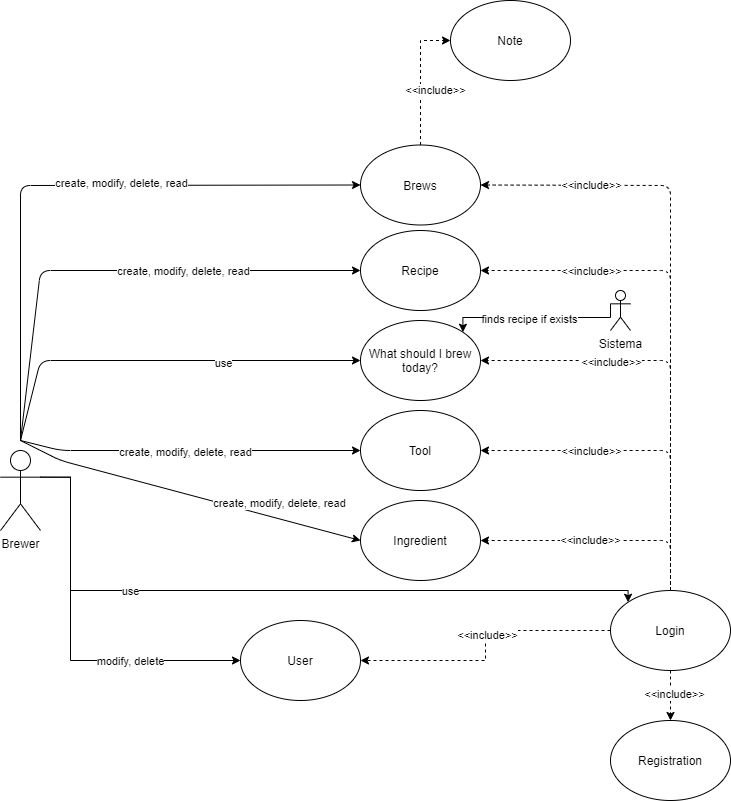
\includegraphics[scale=0.5]{Diagramma casi d'uso.png}
\label{fig:Diagramma Casi d'Uso}
\caption{Diagramma Casi d'Uso}
\end{figure}
\clearpage
\subsection{Diagramma delle classi di dominio}
\begin{figure}[h!]
\centering
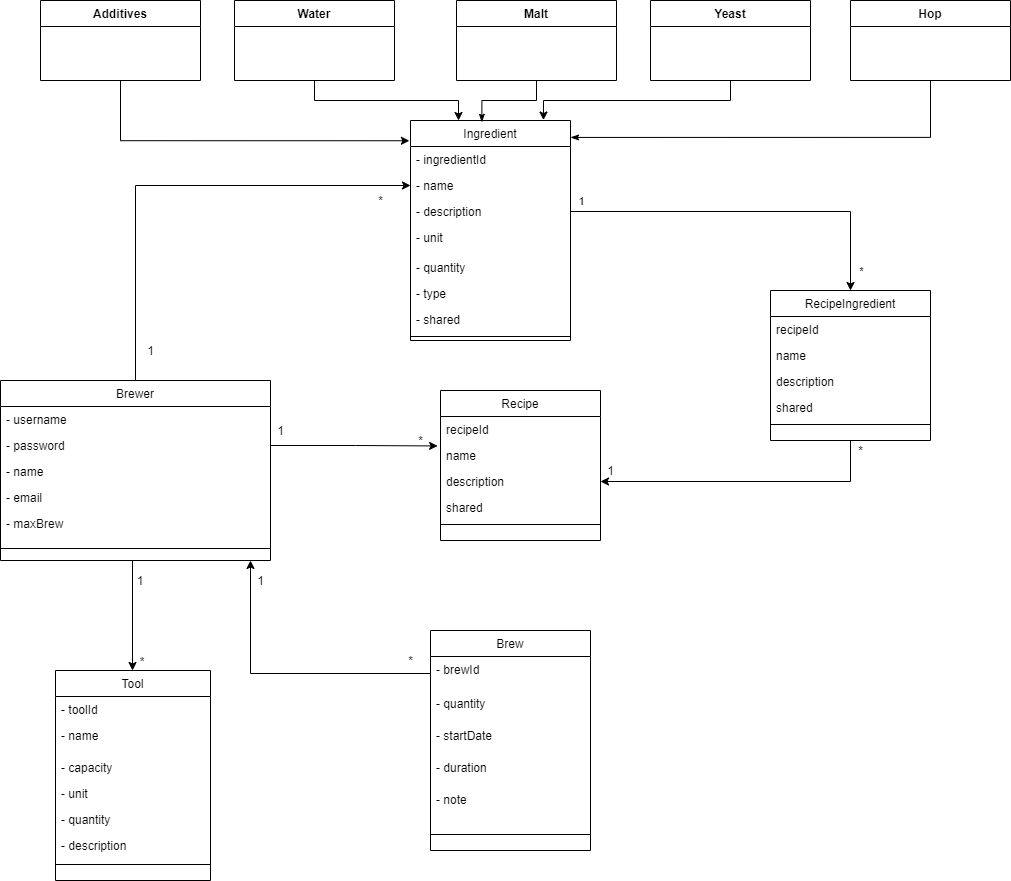
\includegraphics[scale=0.4]{Diagramma di Dominio.png}
\label{fig:Diagramma Casi di Dominio}
\caption{Diagramma Casi di Dominio}
\end{figure}
\clearpage
\subsection{Diagramma SSD (What should I brew today?)}
\begin{figure}[h!]
\centering
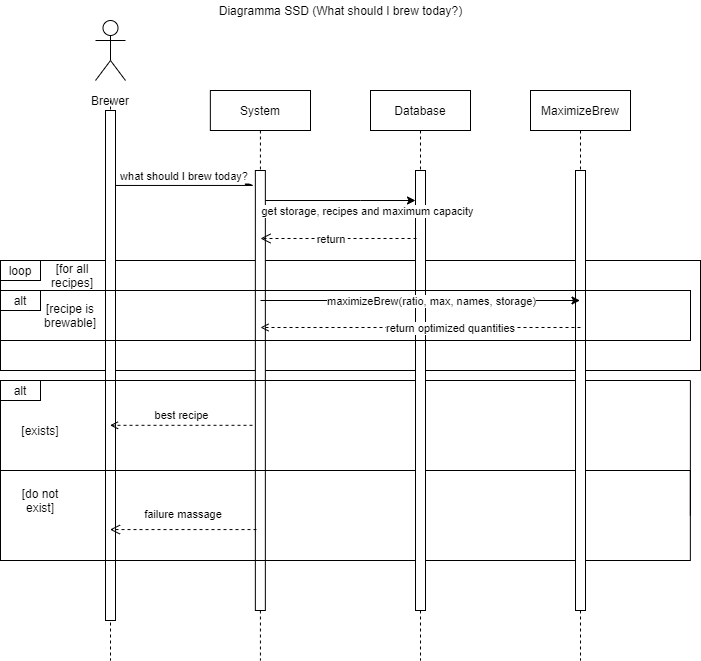
\includegraphics[scale=0.5]{Diagramma SSD (1).png}
\label{fig:Diagramma What should I brew?}
\caption{Diagramma What should I brew?}
\end{figure}
\clearpage
\subsection{Diagramma di sequenza(Creazione ricetta)}
\begin{figure}[h!]
\centering
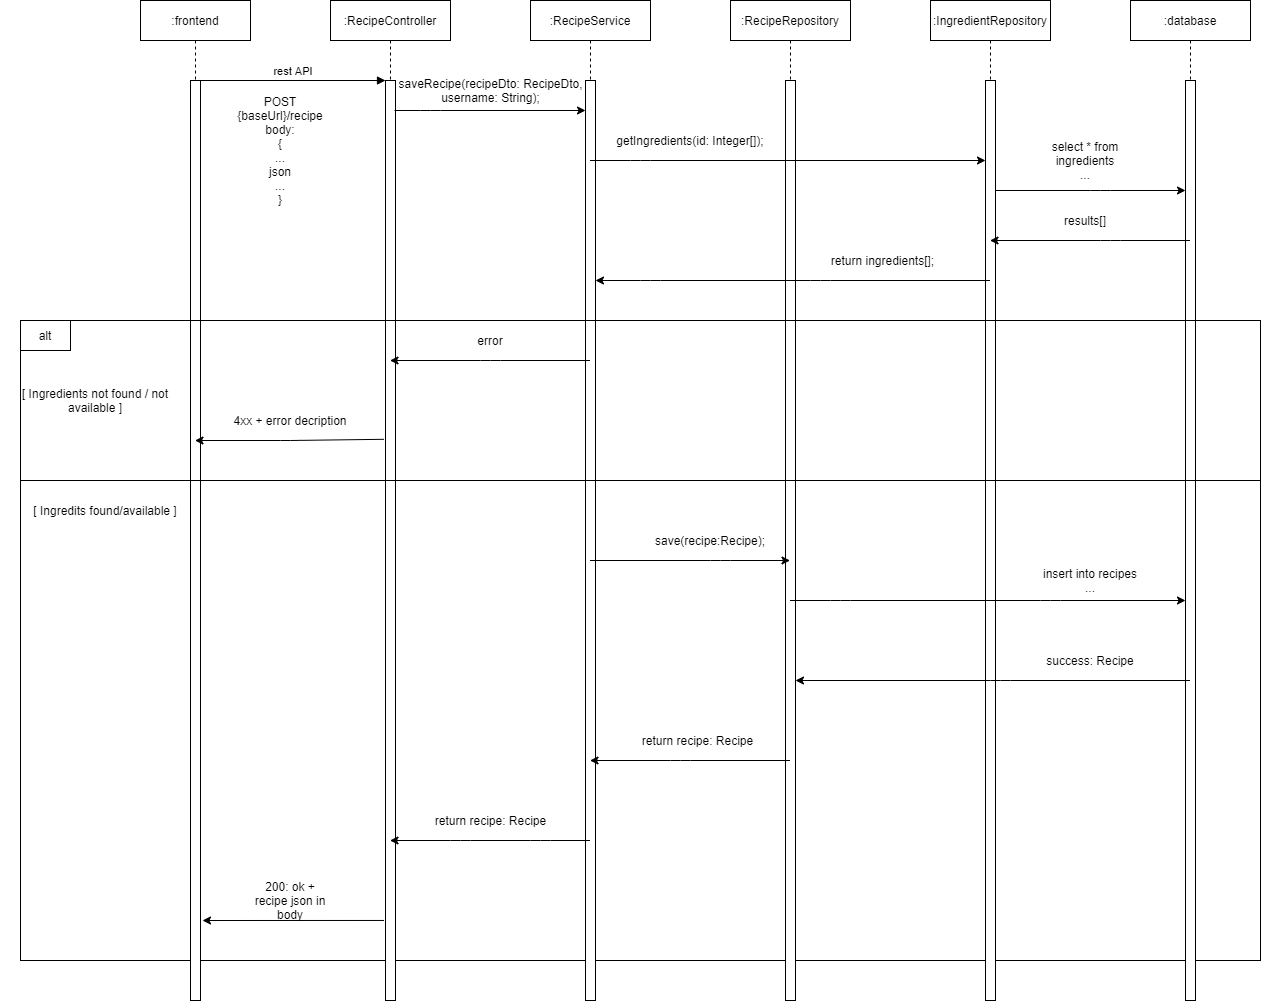
\includegraphics[scale=0.35]{Diagramma di Sequenza (1).png}
\label{fig:Diagramma di sequenza - Creazione ricetta}
\caption{Diagramma di sequenza - Creazione ricetta}
\end{figure}
\clearpage
\subsection{Diagramma delle attività(What should I brew today?)}
\begin{figure}[h!]
\centering
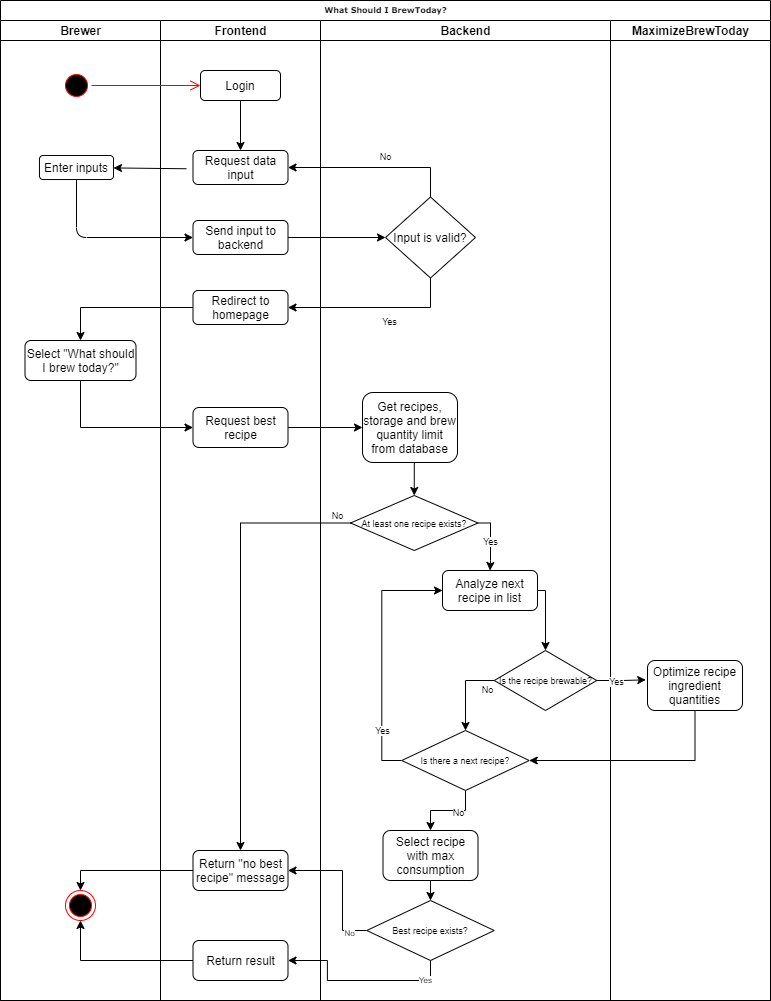
\includegraphics[scale=0.45]{new Activity Diagram.png}
\label{fig:Diagramma di Attività - what should I brew?}
\caption{Diagramma di Attività - what should I brew?}
\end{figure}
\clearpage
\subsection{Diagramma degli stati(Login)}
\begin{figure}[h!]
\centering
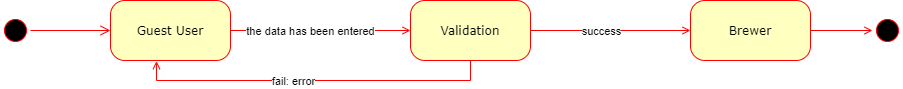
\includegraphics[scale=0.5]{State Diagram_Registrazione (1).png}
\label{fig:Diagramma degli stati}
\caption{Diagramma degli stati}
\end{figure}
Il diagramma di stati è relativo alla fase di Login. Nel momento in cui l’utente deve ancora inserire i dati di accesso (email e password), lo stato
attivo è Utente Ospite fino al momento in cui essi vengono inseriti, successivamente mentre il sistema controlla i dati lo stato è quello di
Validazione. Infine a seconda del risultato:\\
\begin{itemize}
    \item va a buon fine l’utente è loggato e può usufruire delle funzionalità dell’applicazione
    \item non va a buon fine l’utente deve reinserire i dati.
\end{itemize}
\clearpage
\subsection{Diagramma delle classi di progettazione}
\begin{figure}[h!]
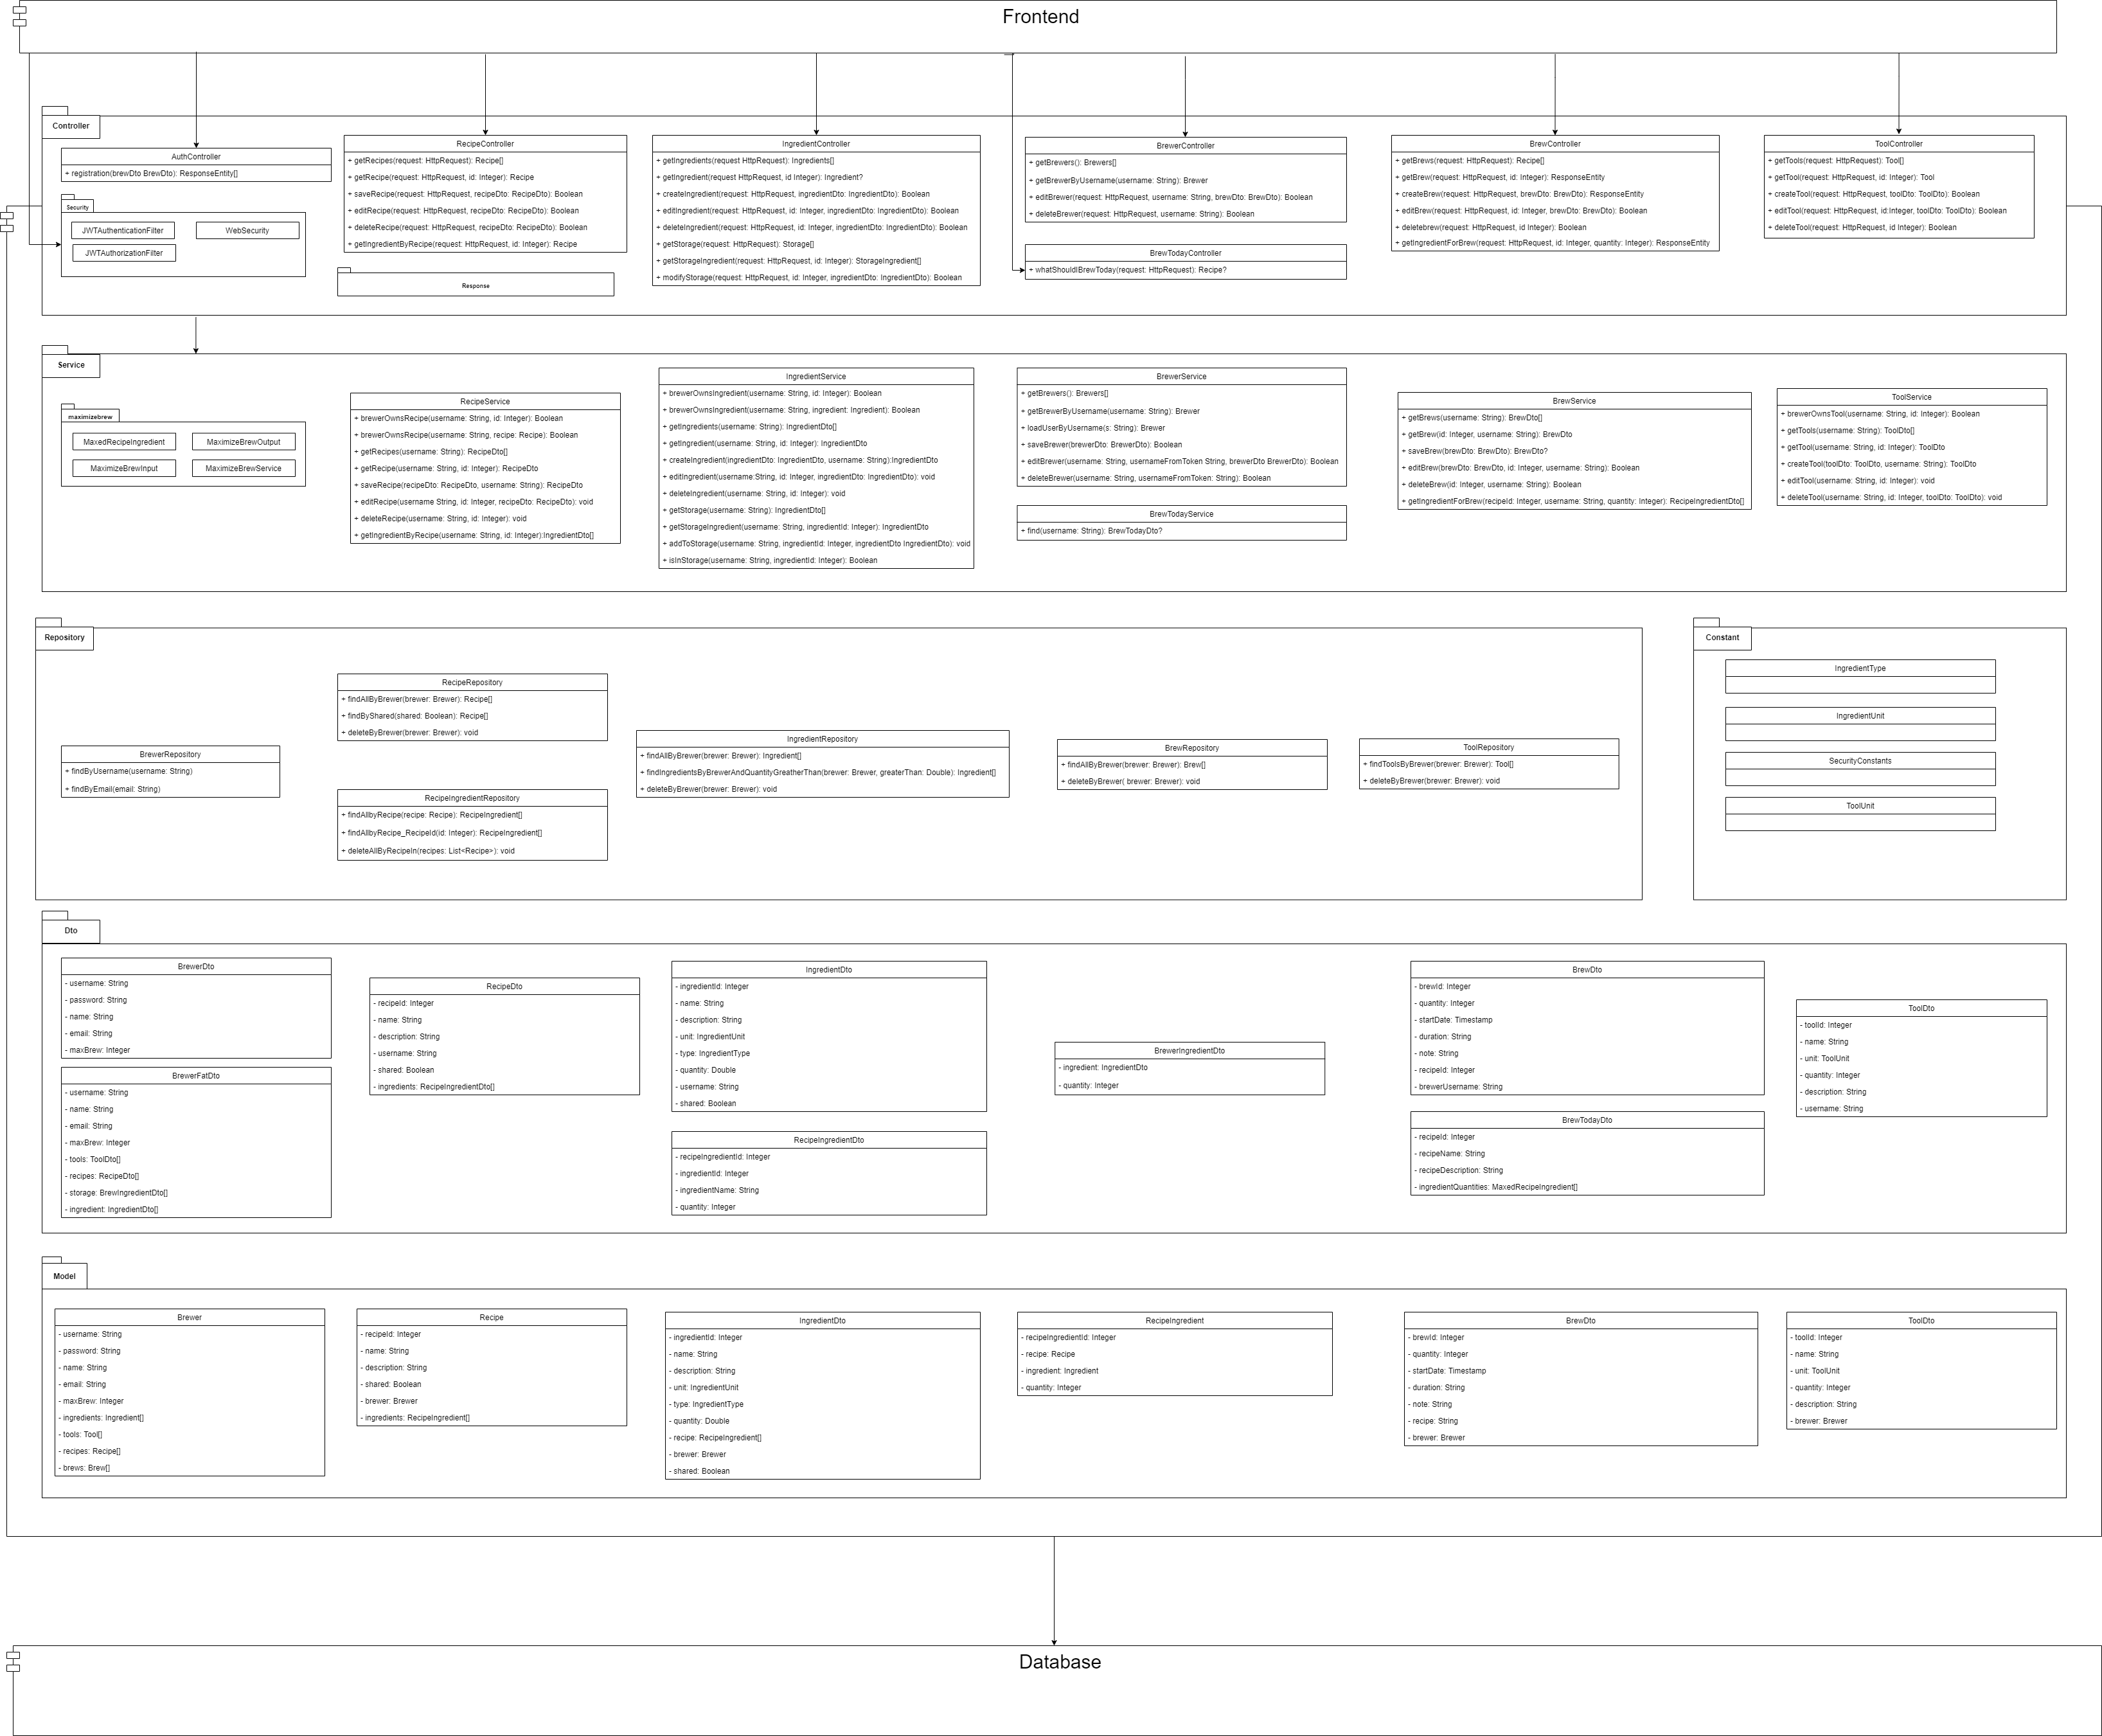
\includegraphics[scale=0.14]{DiagrammaClassiProgettazione-backend.png}
\label{fig:Diagramma classi di progettazione - backend}
\caption{Diagramma classi di progettazione - backend}
\end{figure}
\clearpage
\section{Organizzazione del progetto}
\subsection{Diagramma Gantt}
Per l’organizzazione del progetto e delle sue tempistiche abbiamo utilizzato un diagramma Gantt per poter avere una visione chiara delle attività da svolgere e delle loro tempistiche, in modo da rispettare i tempi di consegna previsti.\\
Dopo un analisi inziale abbiamo delineato alcuni epic/milestone in cui dividere il progetto, ogni macro-attività è stata stimata temporalmente e inserita nel diagramma.\\
Diagramma a inizio progetto:\\
\begin{figure}[h!]
\centering
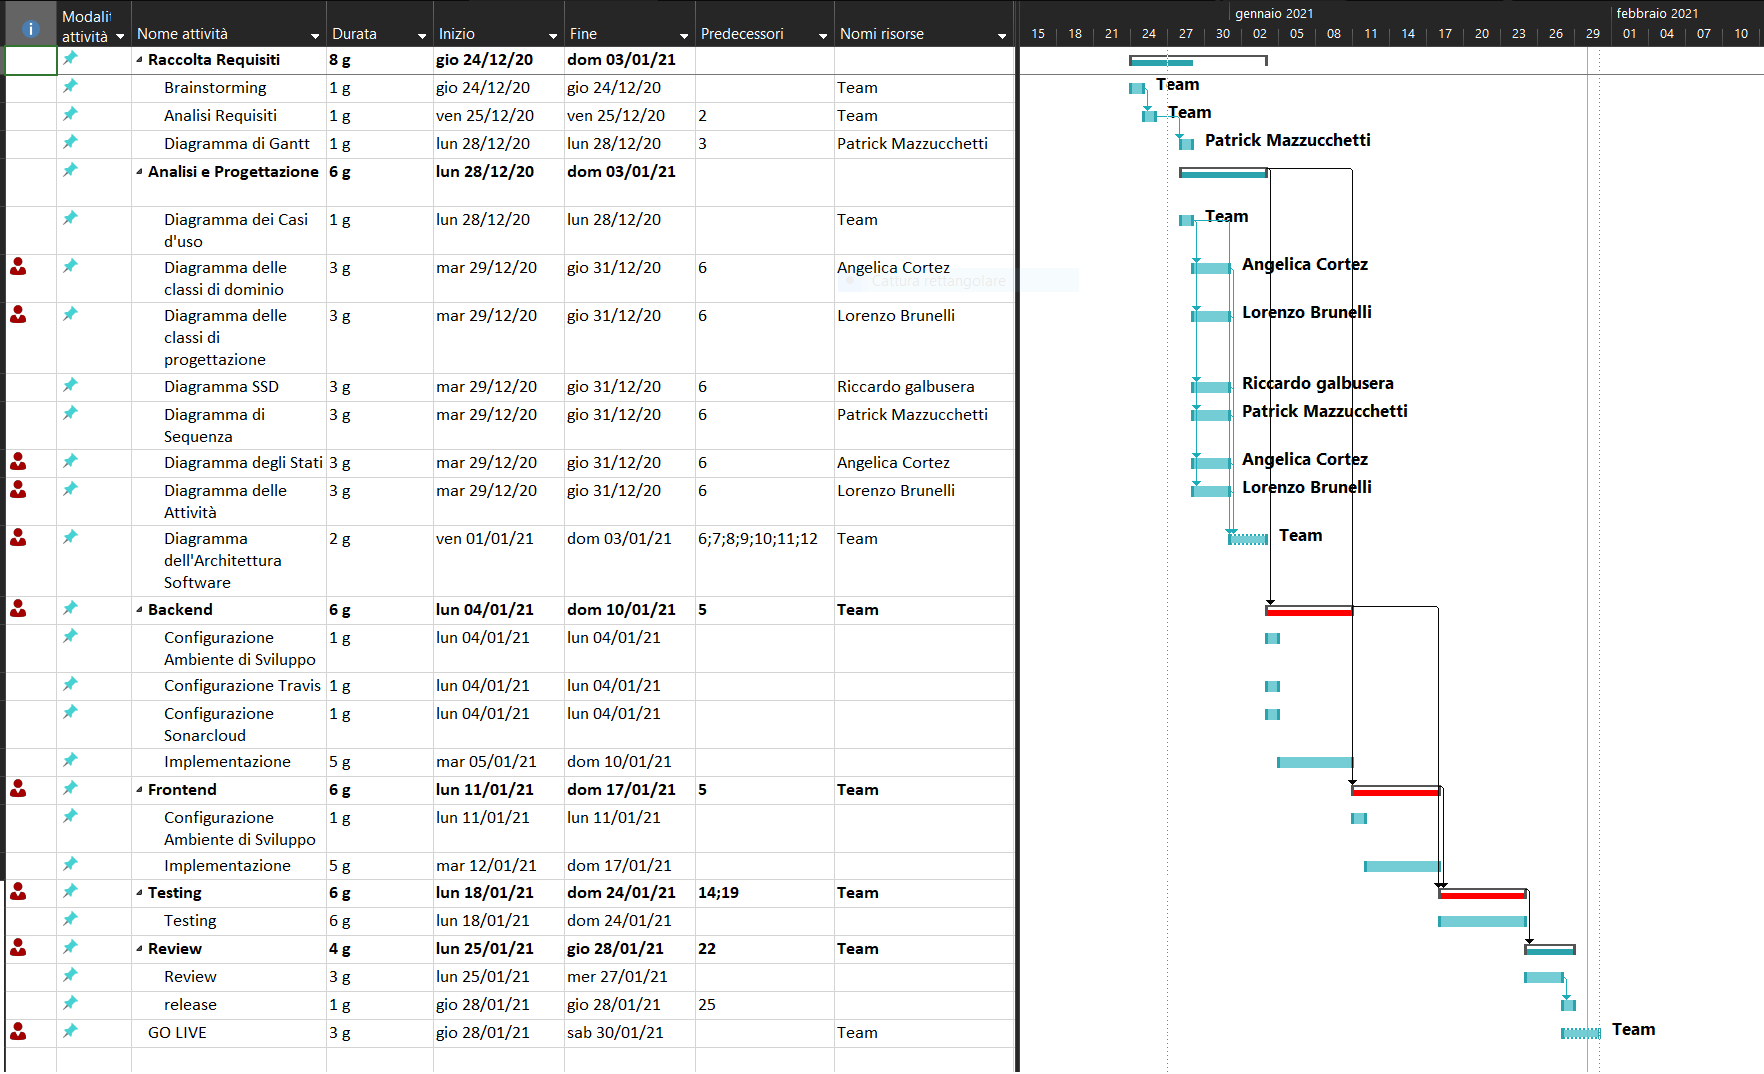
\includegraphics[scale=0.4]{screen1.PNG}
\label{fig:Gantt iniziale}
\caption{Pianificazione del lavoro del team: Gantt}
\end{figure}
\\
A fine progetto le attività sono state svolte effettivamente come indicato nel seguente diagramma Gantt aggiornato:
\begin{figure}[h!]
\centering
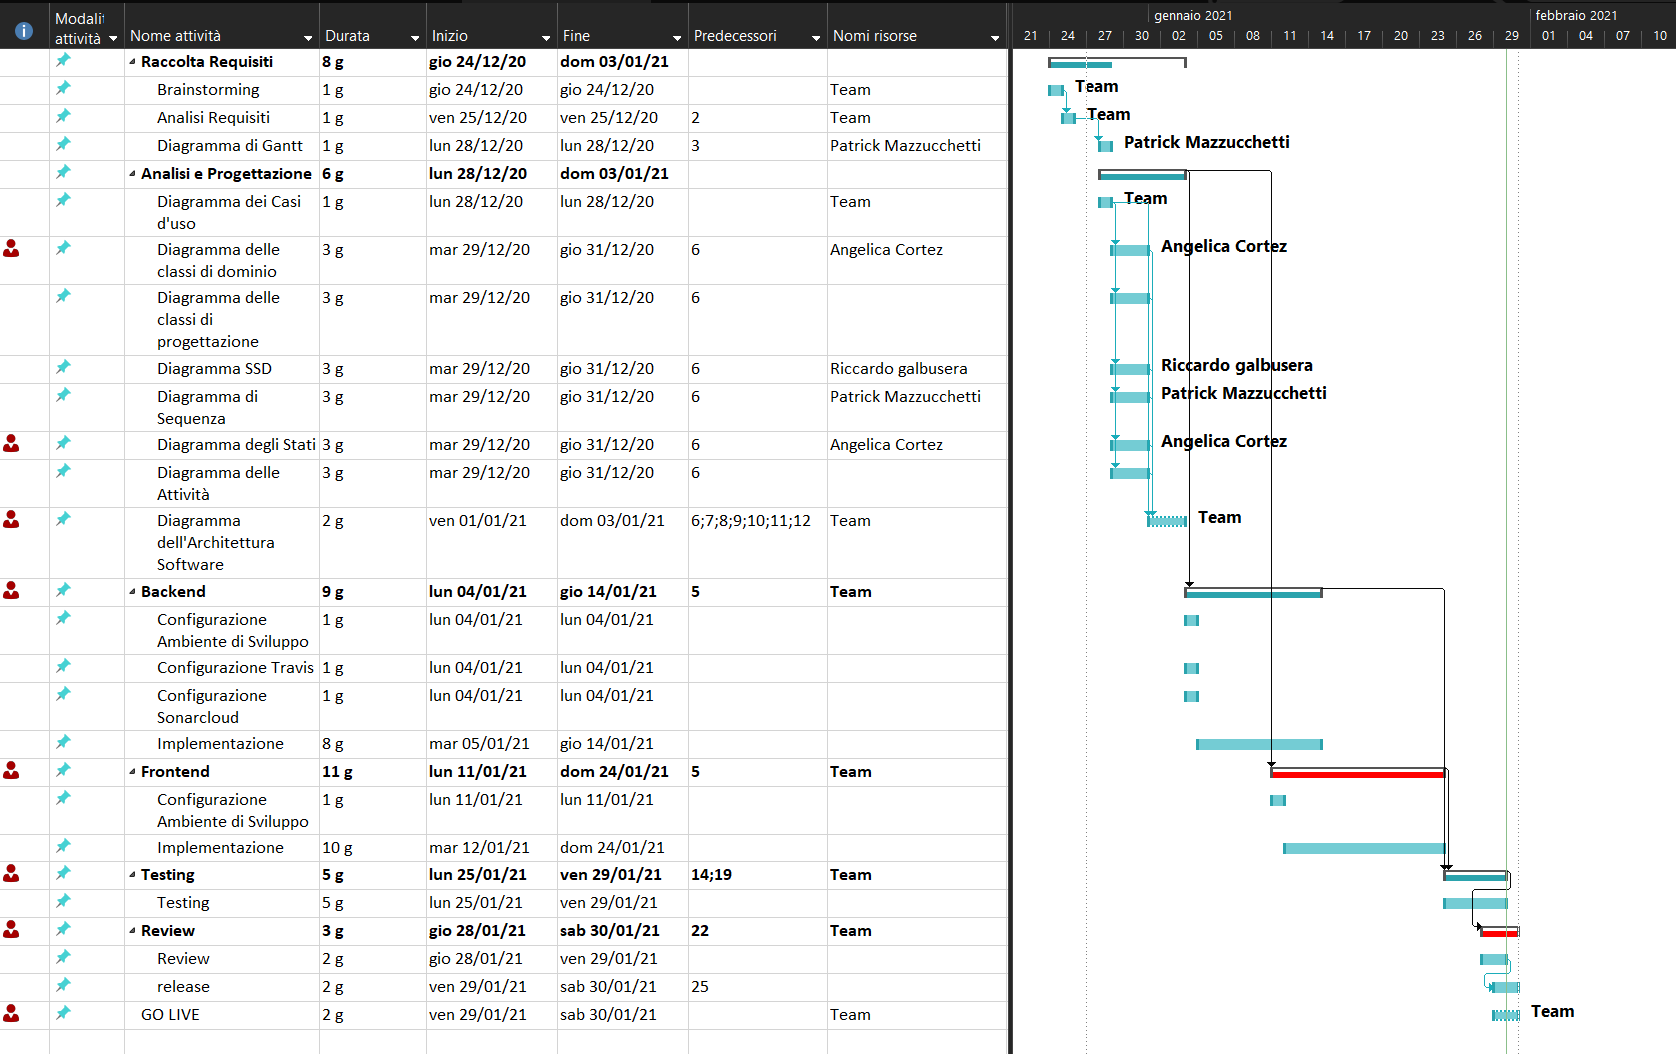
\includegraphics[scale=0.4]{screen1Finale.PNG}
\label{fig:Gantt Finale}
\caption{Concreta Pianificazione del lavoro del team: Gantt Finale}
\end{figure}
\\
Come si evince dal diagramma di Gantt finale, possiamo dire di aver avuto alcune difficoltà a rispettare le tempistiche che ci eravamo prefissati. Abbiamo ritardato nella settimana di backend con un ritardo di ben 4 giorni, con ciò abbiamo dovuto modificare e stringere tutte le tempistiche finendo ad avere 2 giorni di ritardo per la release. Dobbiamo ammettere che i ritardi sono stati causati dalla sovrapposizione della settimana di backend e frontend con il periodo dei compitini ed esami, quindi la fase di implementazione è durata più di quanto fosse previsto.

\subsection{SCRUM}
Per lo svolgimento del progetto abbiamo utilizzato la metodologia SCRUM con sprint di una settimana. A partire dagli epic individuati nella prima fase di analisi abbiamo stabilito le user story e i sottotask da portare a termine in ogni sprint seguendo la programmazione individuata con il Gantt.\\
A supporto della collaborazione del team abbiamo utilizzato la suite di strumenti offerta da Atlassian: Confluence per tutto ciò che ha riguardato la documentazione e Jira per la gestione degli sprint e delle storie utente/ticket.
\clearpage
\section{Implementazione}
\subsection{Gestione repository}
Per la gestione del codice e la collaborazione del team abbiamo utilizzato un repository git su github, come strategia di branching abbiamo deciso di utilizzare il GitFlow così implementato:\\
\begin{itemize}
    \item Abbiamo utilizzato il branch main come ramo principale per il codice stabile da produzione; su questo ramo non abbiamo effettuato push dirette ma abbiamo sempre utilizzato la strategia delle pull request per poter avere una migliore visione globale del codice scritto effettuando review del codice tra di noi e ottenendo informazioni dall’analisi automatizzata effettuata con SonarCloud oltre ai test lanciati da Travis.
    \item Abbiamo utilizzato un branch Develop per il codice invece da testare in un ambiente di sviluppo/staging; come per il branch Main, abbiamo utilizzato il flusso con le pull request per le medesime motivazioni.
    \item Per ogni funzionalità definita dalle user story abbiamo creato un feature branch a partire dal branch di Develop nominato con la chiave del ticket corrispondente su Jira per avere chiaro quale funzionalità si stesse implementando su ogni branch, una volta terminata l’implementazione viene aperta una Pull Request su Develop per poter testare la sua corretta integrazione.\\
    \item I tag di git sono stati utilizzati per tenere traccia delle varie versioni stabili che abbiamo rilasciato.\\
\end{itemize}
Di seguito un diagramma del flusso sulla repository appena descritto:\\
\begin{figure}[h!]
\centering
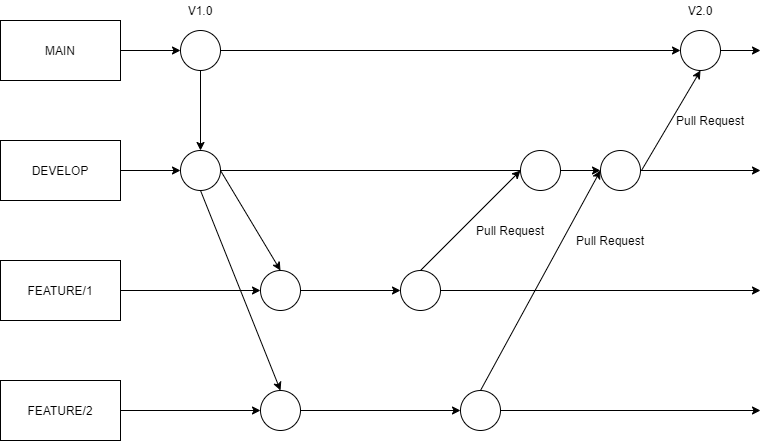
\includegraphics[scale=0.5]{GitFlow.png}
\label{fig:GitFlow}
\caption{GitFlow}
\end{figure}
\subsection{Gestione CI/CD}
\subsubsection{Travis}
Per la gestione del Continuous Integration e Continuous Delivery abbiamo utilizzato lo strumento Travis fornitoci collegato alla nostra repository.\\
Per configurare Travis abbiamo utilizzato un file nominato .travis presente nella root del progetto e lo abbiamo configurato per seguire il seguente flusso:\\
\begin{itemize}
    \item Dopo ogni pull request esclusivamente sui rami Develop e main parte la pipeline di Travis che effettua la build della versione del progetto presente sul ramo nel quale stiamo effettuando la pull request, la build viene effettuata tramite maven che esegue anche i test unitari che abbiamo scritto; una volta andata a buon fine fa partire in automatico l’analisi del codice eseguita tramite SonarCloud.\\
    \item Quando una pull request viene accettata sui rami di Develop e main parta un’altra pipeline di Travis che oltre a verificare che l’integrazione con il codice precedente sia corretta, eseguendo sempre la build del progetto e l’esecuzione dei test unitari, effettua anche il deploy sull’ambiente corretto in relazione al ramo sul quale la pull request viene effettuata.
\end{itemize}
\subsubsection{GitHub Actions}
Nel momento in cui non siamo più stati in grado di utilizzare Travis per la gestione del Continuous Integration e Continuous Delivery abbiamo allora utilizzato lo strumento GitHub Actions fornito da Github.\\
Per configurare le Actions abbiamo utilizzato 3 file posizionati in .github/workflows che specificano il comportamento atteso in seguito alle azioni di push su un branch o l’apertura di una pull request.\\
Abbiamo riportato in questo strumento lo stesso flusso utilizzato con travis: dopo ogni pull request vengono lanciati i test unitari e viene lanciata l’ analisi del codice tramite SonarCloud; quando una pull request viene integrata nei rami di sviluppo o produzione, viene mandato in esecuzione il flusso che effettua il deploy nei nostri ambienti di sviluppo e produzione in base al branch.
\subsubsection{Strategie di deploy}
Nel nostro ambiente di sviluppo le applicazioni sono in esecuzione in container Docker. Per il deploy i container vengono stoppati ed eliminati prima di essere nuovamente creati con le immagini delle nostre applicazioni aggiornate.\\
Nel nostro ambiente di produzione le applicazioni sono in esecuzione su un cluster Kubernetes. Il deploy viene effettuato secondo la strategia del rolling update: quando bisogna eseguire l’update delle immagini dei pod, vengono subito creati nuovi pod con la nuova versione mantenendo però in esecuzione anche quelli con la vecchia versione, una volta che i pod aggiornati sono operativi allora quelli vecchi vengono terminati, permettendo quindi di ottenere un aggiornamento con zero downtime.
\subsection{Gestione analisi qualità del codice}
\subsubsection{SonarCloud}
Per l’analisi della qualità del codice abbiamo utilizzato lo strumento SonarCloud collegato direttamente a Travis/Github Actions e alla nostra repository, abbiamo utilizzato questo strumento per identificare efficacemente possibili problemi nel nostro codice.
\subsection{Infrastruttura}
Per l’infrastruttura a supporto della nostra applicazione ci siamo appoggiati ai servizi Cloud di Amazon AWS.
\subsubsection{Ambiente di Sviluppo}
Per l’ambiente di sviluppo abbiamo utilizzato una EC2 (Elastic Cloud Compute) all’interno di un VPC (Virtual Private Cloud) che manda in esecuzione la nostra applicazione.\\
Essa è raggiungibile dall’esterno tramite SSH sulla porta 22 per la sua configurazione e per la consultazione dei log dell’applicativo e sulla porta 8080 per raggiungere le nostre API, sulla porta 80 per raggiungere il frontend e sulla porta 5000 per raggiungere il microservizio che si occupa della massimizzazione degli ingredienti da utilizzare, al seguente url: \\ \textbf{ec2-52-29-235-197.eu-central-1.compute.amazonaws.com}\\
Sono inoltre presenti dei bilanciatori di carico che permettono il corretto flusso di traffico, interno ed esterno, tra i vari applicativi.\\
Abbiamo anche creato dei record DNS per raggiungere gli applicativi:
\begin{itemize}
    \item \textbf{Frontend:} brewday-dev.progetto-is.com
    \item \textbf{API:} api-dev.progetto-is.com
    \item \textbf{Servizio maximizebrew:} maximizebrew-dev.progetto-is.com
\end{itemize}
All’interno dello stesso VPC è presente anche il servizio RDS (Relational Database Service) che gestisce il nostro database MySql, il database è raggiungibile sulla porta 3306 anche dall’esterno a questo url:\\ \textbf{database-dev.cvmoznlqcyge.eu-central-1.rds.amazonaws.com}\\
\\
Questa scelta è stata fatta per poter lavorare più semplicemente su una base di dati condivisa da tutti i partecipanti del gruppo in sostituzione ad un database locale che avrebbe potuto creare possibili inconsistenze di dati o versioni di MySql effettivamente utilizzate.\\
\begin{figure}[h!]
\centering
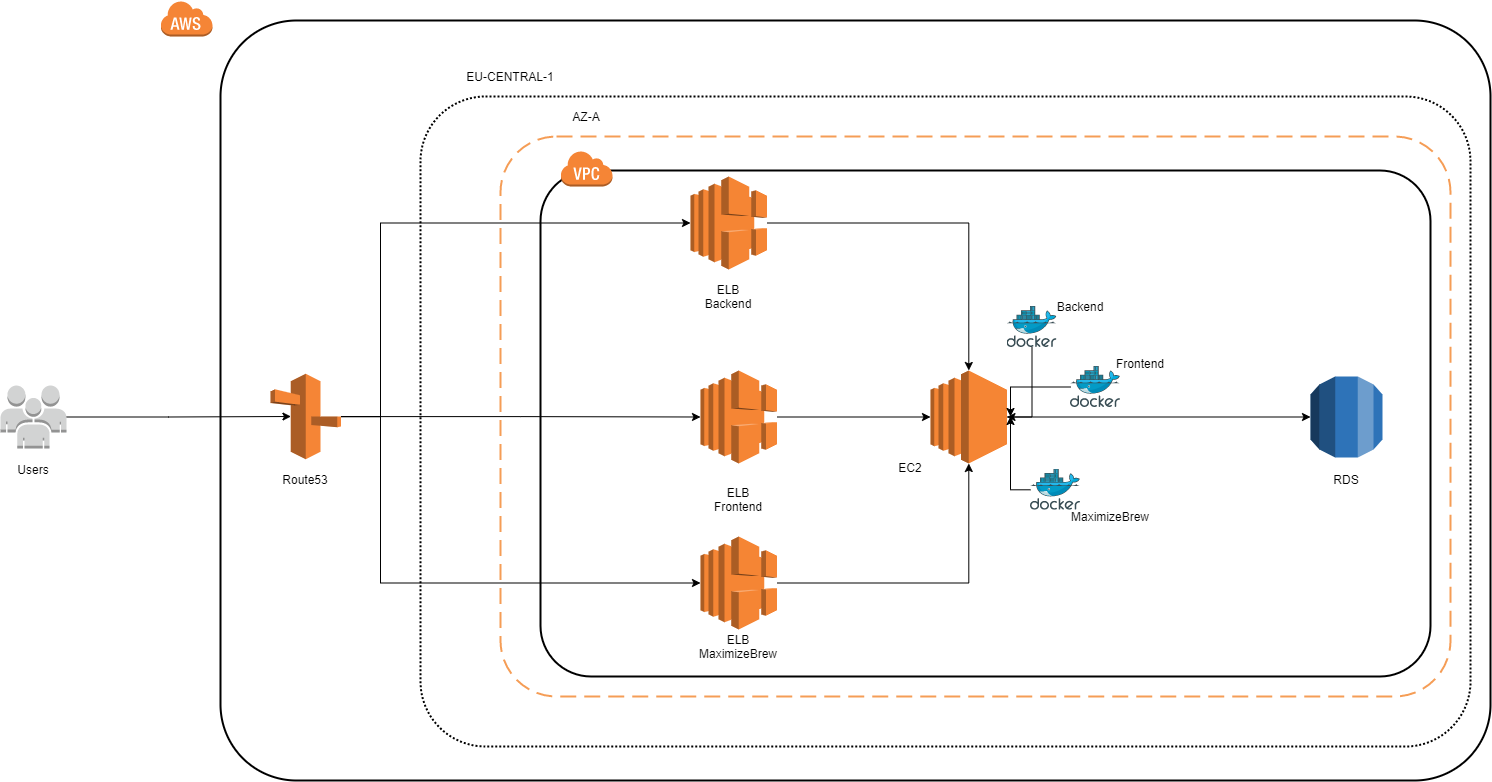
\includegraphics[scale=0.2]{AWS-DEV.png}
\label{fig:AWS-DEV}
\caption{AWS-DEV}
\end{figure}
\clearpage
\subsubsection{Ambiente di produzione}
Per l’ambiente di produzione per garantire prestazioni, affidabilità e disponibilità abbiamo deciso di eseguire le nostre applicazioni all’interno di un cluster Kubernetes gestito tramite il servizio EKS (Elastic Kubernetes Service) di AWS.\\
\\Il nostro cluster si estende all’interno di una Region ma su diverse Availability Zone.\\
Una zona di disponibilità consiste in uno o più data center provvisti di alimentazione, rete e connettività ridondanti in una regione AWS. Le zone di disponibilità consentono ai clienti di eseguire applicazioni e database in ambienti di produzione con elevata disponibilità, tolleranza ai guasti e scalabilità, altrimenti impossibili da ottenere all'interno di un singolo data center.\\
\\
Tutte le zone di disponibilità in una regione AWS sono interconnesse tramite una rete a elevata larghezza di banda e a bassa latenza, su una fibra metropolitana dedicata completamente ridondante che distribuisce reti a alto throughput e bassa latenza tra esse. \\
\\Tutto il traffico tra le zone di disponibilità è crittografato. La prestazione di rete è sufficiente per ottenere una replica sincrona fra le zone di disponibilità. Le zone di disponibilità rendono il partizionamento delle applicazioni per l'alta disponibilità molto semplice. 
\\ \\Il partizionamento di un'applicazione in diverse zone di disponibilità consente l'isolamento delle aziende e le protegge da problemi come blackout, fulmini, tornado, terremoti e altro ancora. Le zone di disponibilità sono fisicamente separate tra loro da una distanza significativa di molti chilometri, pur restando nel raggio di 100 km l'una dall'altra.
\\
Il carico sul cluster viene bilanciato attraverso dei load balancer che si occupano di smistare le richieste al cluster sulle diverse repliche dei nostri applicativi; il cluster inoltre è all’interno di un AutoScaling Group che gli permette di scalare rapidamente, efficacemente e automaticamente in base al carico e alle richieste ricevute.\\ \\
Per il database necessario alla persistenza dei dati ci siamo affidati al servizio RDS con due repliche del database in due zone di disponibilità differenti, un’istanza master e un’istanza solo read che in maniera asincrona viene sincronizzata con l’istanza master; questo oltre che aumentare le prestazioni in lettura dei nostri applicativi garantisce anche backup e failover in caso di problemi.\\
\begin{figure}[h!]
\centering
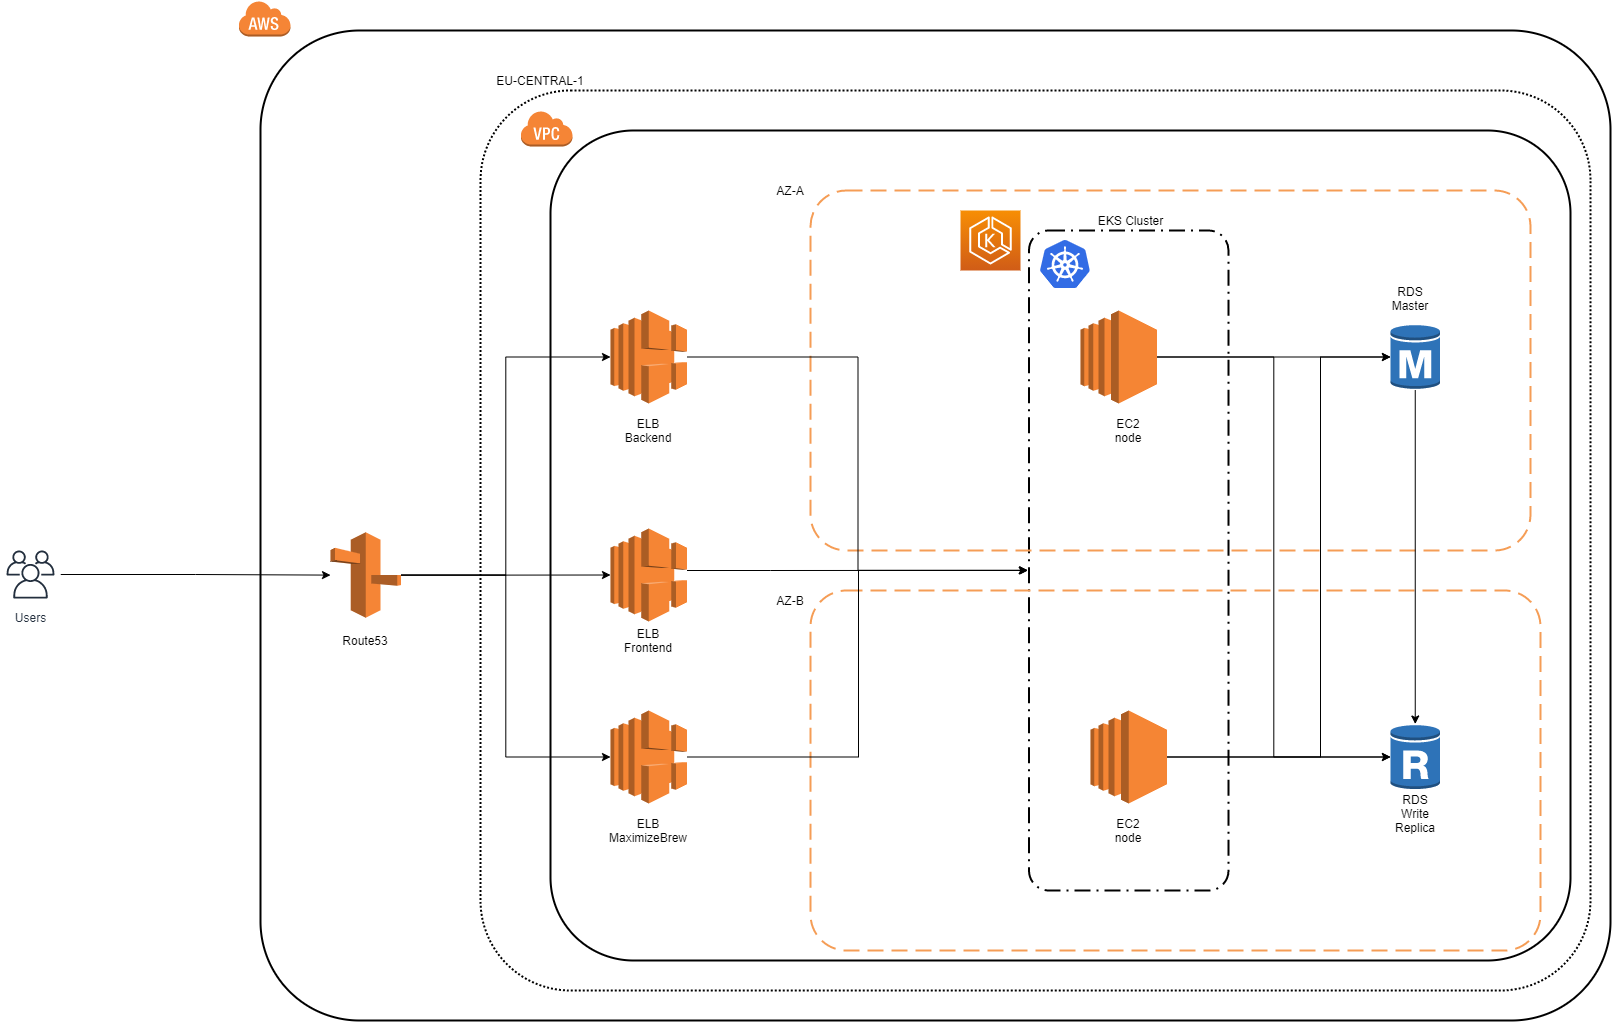
\includegraphics[scale=0.2]{AWS-PROD.png}
\label{fig:AWS-PROD}
\caption{AWS-PROD}
\end{figure}
\clearpage
\subsection{"What Should I brew Today?"}
La classe BrewTodayService contiene la logica necessaria per trovare la ricetta che consuma più ingredienti possibili in dispensa, con relative disponibilità. Per l’ottimizzazione degli ingredienti abbiamo creato un micro servizio in linguaggio python, composto da un’unica classe che sfrutta la libreria di ottimizzazione lineare PuLP, con la quale viene massimizzato il consumo di ingredienti in dispensa.\\
Per ciascuna ricetta avente gli ingredienti necessari in dispensa viene creato un oggetto di input che racchiude le informazioni utilizzate dal micro servizio MaximizeBrewToday, il quale restituisce un oggetto di output contenente le singole quantità per ciascun ingrediente e la loro somma rappresentante il consumo della dispensa.\\
Le ricette vengono mappate al rispettivo valore di consumo in una HashMap e infine viene restituita la ricetta con il valore massimo.\\
Il microservizio espone l’unica API necessaria tramite l’utilizzo del micro framework Flask.
\begin{figure}[h!]
\centering
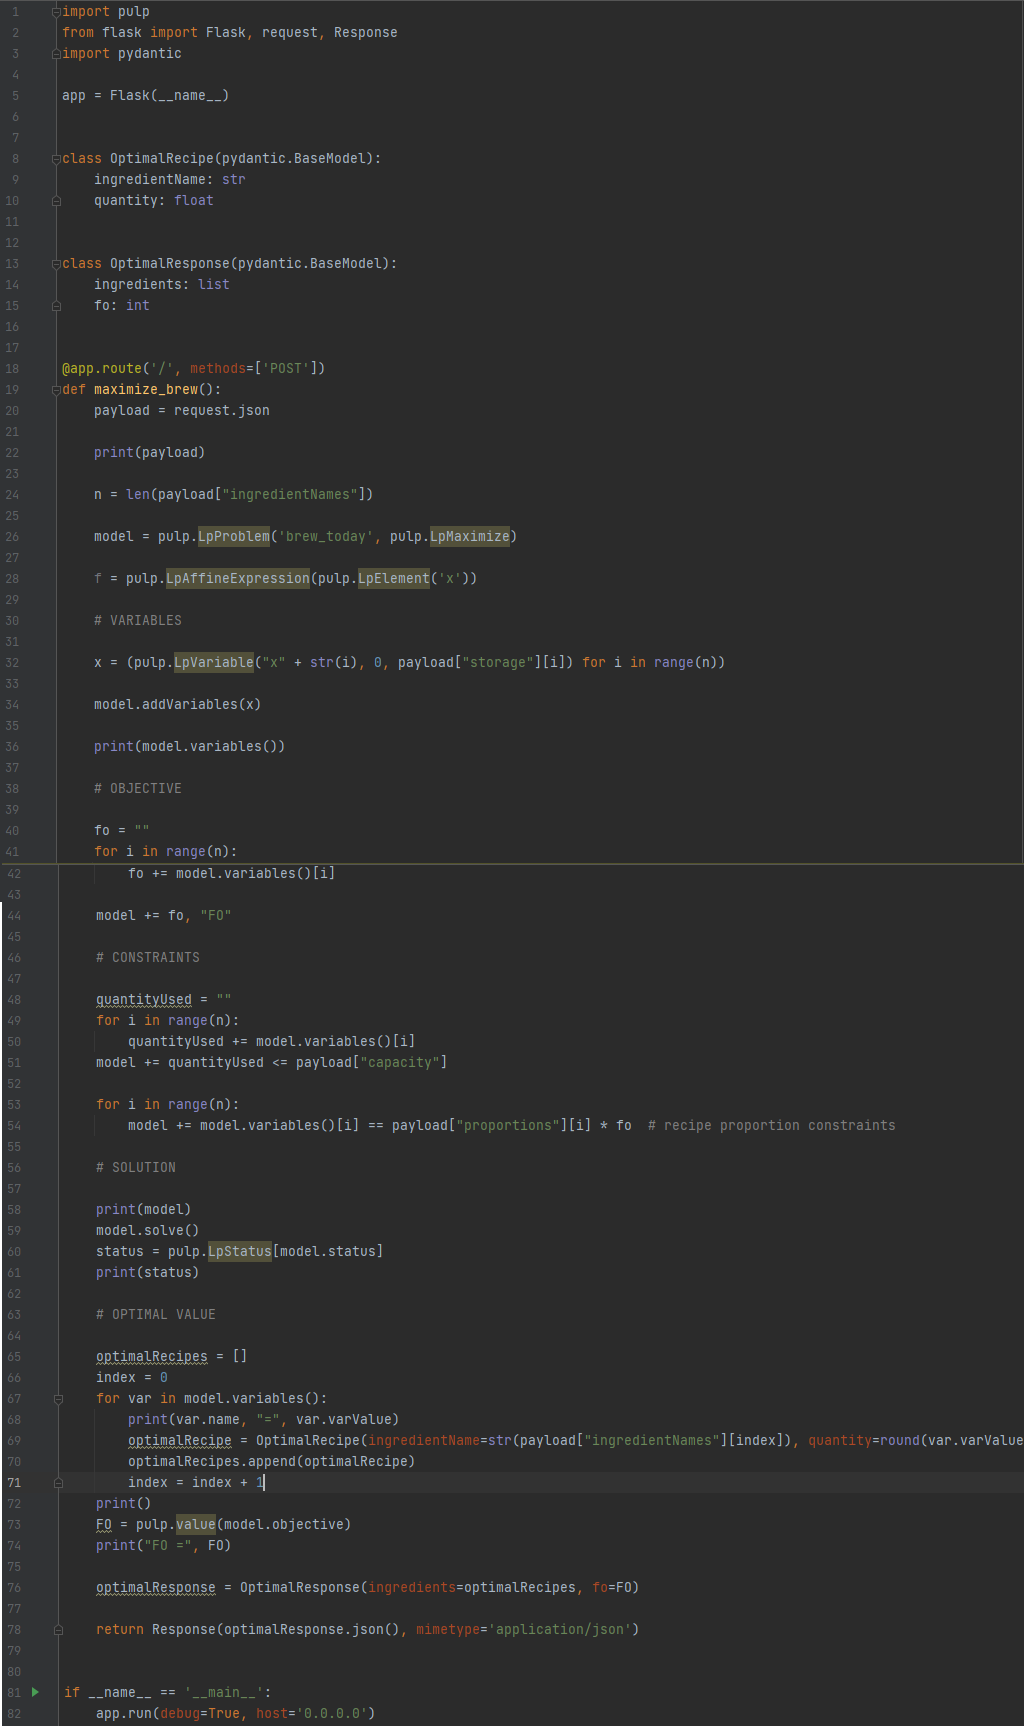
\includegraphics[scale=0.51]{maximize1.PNG}
\label{fig:Codice in python della massimizzazione della funzione obiettivo per la feature}
\caption{Codice in python della massimizzazione della funzione obiettivo per la feature}
\end{figure}
\clearpage
\section{Documentazione backend}
Il backend dell’applicativo è realizzato tramite l’utilizzo del framework Spring, del modulo springboot in particolare, sfruttando anche Hibernate come framework di persistenza.\\
\\
Il progetto è suddiviso in diversi strati seguendo il Pattern MVC e permette di accedere e modificare i dati su un database MySql tramite delle API esposte dall’applicativo.
\begin{figure}[h!]
\centering
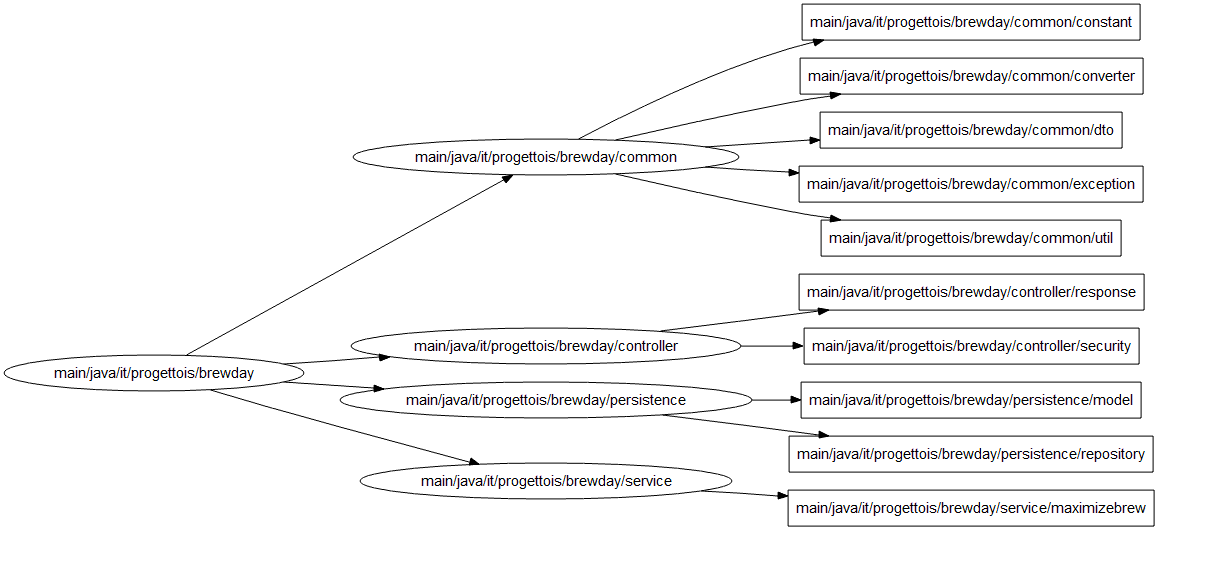
\includegraphics[scale=0.45]{Architecture-brewday.png}
\label{fig:Architettura del BrewDay!}
\caption{Struttura dei package del backend - Brewday!}
\end{figure}
\begin{itemize}
\item \textbf{Strato controller}\\
Le classi implementate in questo strato si occupano di ricevere le chiamate API dall’esterno e di smistarle alla corretta logica applicativa sottostante, si occupano anche di verificare i dati ricevuti in input dall’esterno, dell’autenticazione degli utenti e del ritorno dei corretti messaggi di errore.
\item \textbf{Autenticazione}\\
Tutti gli endpoint esposti (ad eccezione di quello per la registrazione di un nuovo utente) sono protetti, per poterci accedere l’utente deve essere prima autenticato effettuando una chiamata http post all’API “/login” passando all’interno del body della richiesta http username e password, una volta verificato che i dati siano corretti, la chiamata restituisce un token JWT che l’utente dovrà poi inserire nell’header authorization di ogni successiva richiesta.
\item \textbf{Strato Service}\\
Le classi implementate in questo strato si occupano di implementare la logica di business dell’applicativo, in particolare si occupano di convertire i DTO ricevuti dal controller (tramite appositi converter) in entità pronte per essere salvate sul database, di ricevere i dati dal database tramite lo strato di repository e di convertirli in DTO da restituire al controller, e di aggregare e formattare i dati ricevuti da tabelle diverse in modo da portare a termine la corretta logica richiesta.
\item \textbf{Strato persistence}\\
In questo strato sono presenti le interfacce repository implementate per occuparsi della persistenza dei dati sul database e le classi model che servono a mappare le tabelle presenti sul database in entità utilizzabili secondo una logica ad oggetti.
\end{itemize}
\clearpage
\section{Documentazione frontend}
L’interfaccia utente è stata realizzata tramite l’utilizzo del framework Angular, il quale sfrutta il linguaggio TypeScript, un super-set di istruzioni JavaScript. Anche in questo caso vi è una suddivisione a strati.
\begin{itemize}
    \item \textbf{Strato Service}\\
Questo è lo strato che effettua le varie richieste HTTP alle API. E' quindi lo strato che fa da ponte tra la componente di frontend a quella del backend.\\
Tutte le chiamate HTTP sono effettuate in maniera asincrona in modo non bloccante, permettendo all’applicativo di continuare a funzionare anche durante una chiamata, sfruttando il pattern Observer.
\item \textbf{Strato Model}\\
Nello strato del model sono presenti le classi che rappresentano gli oggetti ricevuti in risposta dalle API come JSON al loro tipo specifico (ricette, ingredienti..).
\item \textbf{Strato Component}\\
Nello strato component sono presenti tutti i componenti che rappresentano le varie viste della nostra interfaccia grafica, in particolare tutti i form per inserire nuove entità, le tabelle per la visualizzazione dei dati raggruppati (filtrabili e ordinabili) e le viste per visualizzare il dettaglio di ogni singola entità.\\
Ogni componente è composto da 3 file sorgenti, uno per lo stile css personalizzabile in maniera indipendente, uno contenente il codice html da visualizzare e infine un file TypeScript dove viene specificata la logica del componente.
\end{itemize}
\section{Documentazione API}
La documentazione delle API esposte è stata realizzata tramite l’integrazione nel nostro progetto di Swagger UI, accessibile ai seguenti indirizzi:
\begin{itemize}
    \item Sviluppo: https://api-dev.progetto-is.com/swagger-ui.html
    \item Produzione: https://api.progetto-is.com/swagger-ui.html
\end{itemize}
\clearpage
\section{Design Pattern}
Tutte le classi che vengono utilizzate secondo la funzionalità dell’autowired fornita da Spring sono istanziate secondo un’implementazione particolare del Singleton.\\
\subsection{Observable}
Il pattern viene utilizzato nel frontend per effettuare chiamate asincrone. Attraverso il metodo subscribe si attende la risposta dalle API mentre il resto del programma può continuare la propria esecuzione, permettendo di caricare parte dell’interfaccia utente prima ancora di ricevere indietro i dati richiesti.
\subsection{DTO}
Abbiamo deciso di utilizzare il pattern dei Data Transfer Object per separare gli oggetti nello strato di persistenza dai dati che sarebbero stati inviati e ricevuti nello strato di controller. Lo strato di service si occupa di chiamare i converter, classi utilizzate proprio per convertire un oggetto in dto e viceversa.
\subsection{Builder}
L’implementazione del builder viene effettuata dalla libreria Lombok, è infatti sufficiente inserire la notazione @Builder sopra ad una classe perché questi vengano implementati automaticamente. Abbiamo utilizzato il pattern nelle classi Dto così da poter essere sfruttati nei relativi converter. Sono stati anche utili ai fini del testing, facilitando la comprensibilità nella creazione delle istanze.
\subsection{Repository} 
Il pattern repository viene utilizzato nel backend per implementare la separazione dei problemi astraendo la logica di persistenza dei dati nella web application. E' uno dei desgin pattern più comunemente utilizzati per risolvere problemi ricorrenti.
\clearpage
\section{Design Pattern Architetturali}
\subsection{MVC}
Abbiamo costruito l'architettura sul modello MVC. Abbiamo scelto questo design pattern perchè può essere sviluppato contemporaneamente e consente il raggruppamento logico delle azioni correlate su un controller insieme. Le viste per uno specifico modello sono raggruppati insieme, il che ha una coesione davvero elevata quindi è molto stabile. È facile da sviluppare e modificare in futuro, a causa della separazione delle responsabilità. I componenti del sistema sono anche riusabili e possono essere utilizzate altrove senza e/o con poche modifiche.
\begin{figure}[h!]
\centering
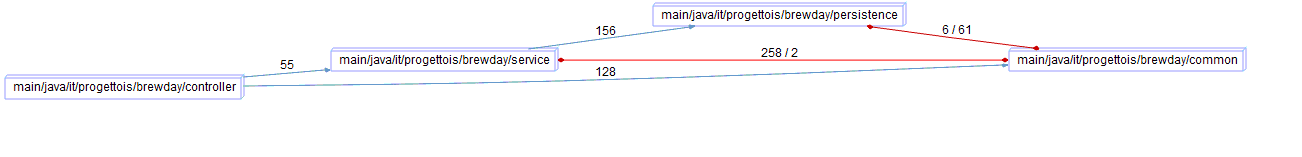
\includegraphics[scale=0.5]{ArchInternalDependencies-brewday.png}
\label{fig:Diagramma delle dipendenze tra i package nel backend}
\caption{Diagramma delle dipendenze tra i package nel backend}
\end{figure}
\subsection{Microservice}
La funzione “What should I brew today?“ utilizza un micro servizio in ascolto sulla porta 5000. Questo è un applicativo python composto da una sola classe che si occupa di massimizzare le quantità di ingredienti utilizzate da una ricetta.
\subsection{Interceptor}
Abbiamo utilizzato il pattern interceptor nella parte del frontend per poter interecettare ogni chiamata http effettuata dai vari service e inserire nella chiamata il token JWT necessario per l’autenticazione.\\
L’utilizzo di questo pattern ci ha permesso di non dover ripetere la stessa logica in ogni chiamata e ci ha dato la possibilità di eseguire automaticamente e in maniera transaparente questa operazione su ogni servizio.  \\
\section{Overview - Principi}
Per la creazione della web application ci siamo basati su alcuni principi tra cui alcuni riportati qui sotto.
\subsection{Principi SOLID}
Abbiamo utilizzato i principi SOLID affinchè lo sviluppo della nostra web application fosse estendibile e mantenibile, in particolare nel contesto di  uno sviluppo agile e fondato sull’identificazione di code smell e sul refactoring.\\
La parola SOLID è un acronimo che serve a ricordare tali principi (Single responsibility, Open-closed, Liskov substitution, Interface segregation, Dependency inversion).
\subsubsection{Single-responsiblity principle}
\textit{"A class should have one and only one reason to change, meaning that a class should have only one job."} \\
Il principio afferma che ogni classe dovrebbe avere una ed una sola responsabilità, interamente incapsulata al suo interno. Non avendo delle istruzioni precise su come implementare questo principio, abbiamo dato un interpretazione personale sulle responsabilità di ciascuna classe. Esempio la classe Tool gestisce SOLO gli strumenti che ha il brewer nel suo inventario oppure la classe Ricetta che gestisce SOLO le ricette possedute.
\subsubsection{Open-closed principle}
\textit{"Objects or entities should be open for extension, but closed for modification."}
Questo principio è stata utilizzata molto durante la progettazione, un esempio può essere la creazione di un eccezione universale "GenericNotFoundException" che è aperta alle estensioni (quali: NoBestRecipeException, IngredientNotFoundException, ToolNotFoundException,...) ma chiusa alle modifiche.
\subsubsection{Liskov substitution principle}
\textit{"Let q(x) be a property provable about objects of x of type T. Then q(y) should be provable for objects y of type S where S is a subtype of T.}\\
Anche questo principio, che si basa sul corretto uso dell’ereditarietà, è stato molto utilizzato durante la progettazione, ad esempio nella gestione delle eccezioni, come descrito sopra; ogni eccezione specifica è un sottotipo di un altro oggetto più generico ma il comportamento resta corretto qualisasi dei due oggetti si scelga di utlizzare. Nella sezione frontend tutte le classi Service estendono anche qua una classe più generica; le azioni della nostra tabella si basano su questo principio: richiamano metodi presenti nel generic service aspettandosi di eseguirli su sottotipi specifici senza alterarne la correttezza.
\subsubsection{Interface segregation principle}
\textit{"A client should never be forced to implement an interface that it doesn’t use or clients shouldn’t be forced to depend on methods they do not use."}\\
Ci siamo basati su questo principio creando un interfaccia dinamica personale per il brewer a seconda delle sue esigenze.
\subsubsection{Dependency Inversion Principle}
\textit{"Entities must depend on abstractions not on concretions. It states that the high level module must not depend on the low level module, but they should depend on abstractions."}\\
Abbiamo creato moduli di alto livello che non devono dipendere da quelli di basso livello, ad esempio, abbiamo creato una classe BrewerService che implementa i metodi findByUsername() e findbyEmail(), che recuperano le informazioni dell'utente dal livello di persistenza utilizzando una semplice implementazione repository. In questo caso, il tipo BrewerRepository è l'astrazione che BrewerService utilizza per consumare il componente di basso livello.
\clearpage
\subsection{PHAME} 
Ci siamo anche appoggiati ai principi di progettazione del software PHAME, quali i principi di gerarchia, astrazione, modularizazzione e incapsulamento riassunta nella foto sottostante.
\begin{figure}[h!]
\centering
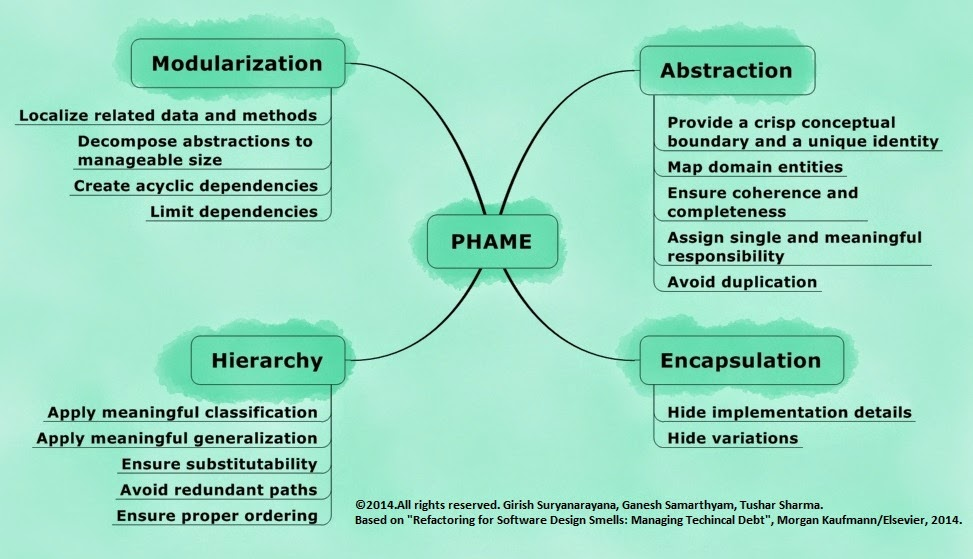
\includegraphics[scale=0.4]{PHAME.jpg}
\label{fig:PHAME}
\caption{Design Principles PHAME}
\end{figure}
\\
\section{Procedura di installazione: On-premises o SAAS}
Per come si sta evolvendo il mondo dell’informatica e dell’ormai onnipresenza di software forniti come servizi, abbiamo deciso di implementare il nostro progetto secondo questa filosofia SAAS.\\
\\
La maniera più semplice e intuitiva quindi per poter fruire della nostra applicazione è quella di sfruttare la sua versione in cloud e accederci tramite l’url: https://brewday.progetto-is.com che porta direttamente alla nostra infrastruttura di produzione su AWS; è anche il modo principale con cui ci aspettiamo che i nostri ipotetici clienti utlizzeranno la nostra applicazione.\\
\\
A scopo di test o di sviluppo è possibile eseguire in locale l’applicazione o parte di essa seguendo una delle seguenti modalità.
\subsection{Docker Compose}
Requisiti:
\begin{itemize}
\item Docker
\item Docker-compose
\end{itemize}
\begin{enumerate}
    \item Dalla root del progetto eseguire il comando docker-compose up
    \item Il comando si occuperà di scaricare le immagini da docker hub e manderà in esecuzione tutto l’ambiente.
    \item Il frontend sarà accessibile sulla porta 4200 tramite browser
    \item Il database inzialmente sarà vuoto quindi la prima operazione da fare sarà quella di eseguire la registrazione dal frontend.
\end{enumerate}
\subsection{Effettuare il build delle immagini docker direttamente dai sorgenti (Opzionale)}
Requisiti: 
\begin{itemize}
    \item Docker
    \item Maven
\end{itemize}
\subsubsection{Backend:}
Dalla root del progetto
\begin{enumerate}
    \item cd backend
    \item mvn clean install (Aggiungre -DskipTests=true per saltare i test unitari)
    \item docker build -f Dockerfile-compose -t gruppobirra2/brewday:local .
\end{enumerate}
\subsubsection{Maximizebrew:}
Dalla root del progetto
\begin{enumerate}
\item cd maximizebrewtoday 
\item docker build -t gruppobirra2/maximizebrewtoday:local .
\end{enumerate}
\subsubsection{Frontend:}
Dalla root del progetto
\begin{enumerate}
\item cd frontend
\item docker build -t gruppobirra2/brewday-frontend:local .
\end{enumerate}
\subsection{Lanciare l'analisi della qualità del codice con SonarCloud}
Dalla root del progetto
\begin{enumerate}

\item cd backend

\item mvn clean org.jacoco:jacoco-maven-plugin:prepare-agent install sonar:sonar\\ -Dsonar.projectKey=UnimibSoftEngCourse2021$_$progetto-birra-2-gruppo-birra-2`
\end{enumerate}
\end{document}
